%\documentclass{acm_proc_article-sp} 
\documentclass[14pt]{article} 
\usepackage{amssymb,amsmath} 
\usepackage{setspace}
\usepackage{graphicx}
\usepackage{float}
\usepackage{hyperref}

\doublespacing


%\floatstyle{ruled}
%\newfloat{code}{thp}{lop}
%\floatname{code}{Code}

%\DeclareGraphicsExtensions{.eps}

\begin{document}
	
\title{DBToaster Runtime: A System for Streaming Data Processing. \\And\\ AlgoTrader: A Trading Algorithms Platform for Stock Exchange Simulation.}
\author{Anton Morozov}
\maketitle

\section{Introduction}

DBToaster Runtime is a system build based on DBToaster. Runtime provides a stand alone interface for execution of user defined, DBToaster compiled queries over specified update streams. Capabilities and usage of the system are demonstrated on an example of AlgoTrader. AlgoTrader is a platform that simulates Stock Exchange and serves as a testbed for automatic Trading Algorithms.   

DBToaster Runtime can be partitioned into three major components: Compiler, Data Sources Processor and Query Processor. Compiler receives SQL queries from a client, compiles them down to executable code and passes to Query Processor for execution. Data Sources Processor manages a set of update data streams and passes data to appropriate queries in Query Processor. Query Processor runs a set of queries over given data. The results of each query are made available to connected clients. 

AlgoTrader platform provides an example of how an application over update streams can benefit form DBToaster Runtime. AlgoTrader is a time critical application, which uses expressive set of queries over update streams. The platform consist of two components: Stocks Exchange Simulator and Trading Algorithms Engine. Stock Exchange Simulator implements a realistic simulation of an Electronic Communication Network (ECN). Each ECN serves as a matchmaker between stock buyers and sellers. Trading Algorithms Engine is a testbed for developing automatic trading strategies. Each strategy runs a set of queries over a data stream(s) coming from Stock Exchange Simulator. Based on query results trading strategies either buy or sell stocks.

Interactions between DBToaster Runtime and AlgoTrader can be seen in figure \ref{TheBigPicture}.


%Data Sources components are a source of the incoming data. The end user applications need these data to be processed by running various queries over it. In this particular example we will be using an Exchange Simulation Server application as a data source. Next component is the Algorithms Simulation Engine. This component is the end user program of interest. It is responsible for the decision making and outside influences (i.e. what ever user needs to be done with the help of the queries over the data streams). In out example it is a Trading Runtime Platform. The last component is DBToaster Runtime. The component is responsible for collecting the data from various data sources specified by the users, running appropriate queries over the data and conveying the query results to Algorithms Simulation Engine. 

%The the flow of information between the three components is as follows. Once started data generation component generates data, these data comes from a variety of sources stock exchange, sensor network, remote applications etc. The data comes as a continuous stream of information, this information is presented in a well known format. In many of the cases it is possible that the end user does not have much control over the data stream but the ability to listen to the incoming data. These data is sent to DBToaster runtime. The runtime is responsible for collecting data from those data sources and running a dynamic set of user defined queries over these data. The queries are dynamically loaded, compiled and if needed removed during the execution of a runtime. The results of the queries are forwarded to Algorithms Simulation Engine (a.k.a the end user). The Engine's job is to get the data from the runtime. Based on the results of the queries Algorithm Engine performs tasks needed by the users. In our example, based on the information received Algorithm Engine buys and sell stocks on a NASDAQ exchange simulator. 

%The particular application we have chosen to demonstrate the capabilities and performance of our system is a NASDAQ trading simulation. In this simulation there is a set of servers; each server arranges stock exchanges between different trading parties. The results of those exchanges as well as information about interest in stock sells and purchases is transmitted to all parties interested in such information. Based on these information different trading algorithms decide to buy and sell stocks. The arrangement of all the components in the Trading system can be seen in figure \ref{TheBigPicture}. 

\begin{figure}
  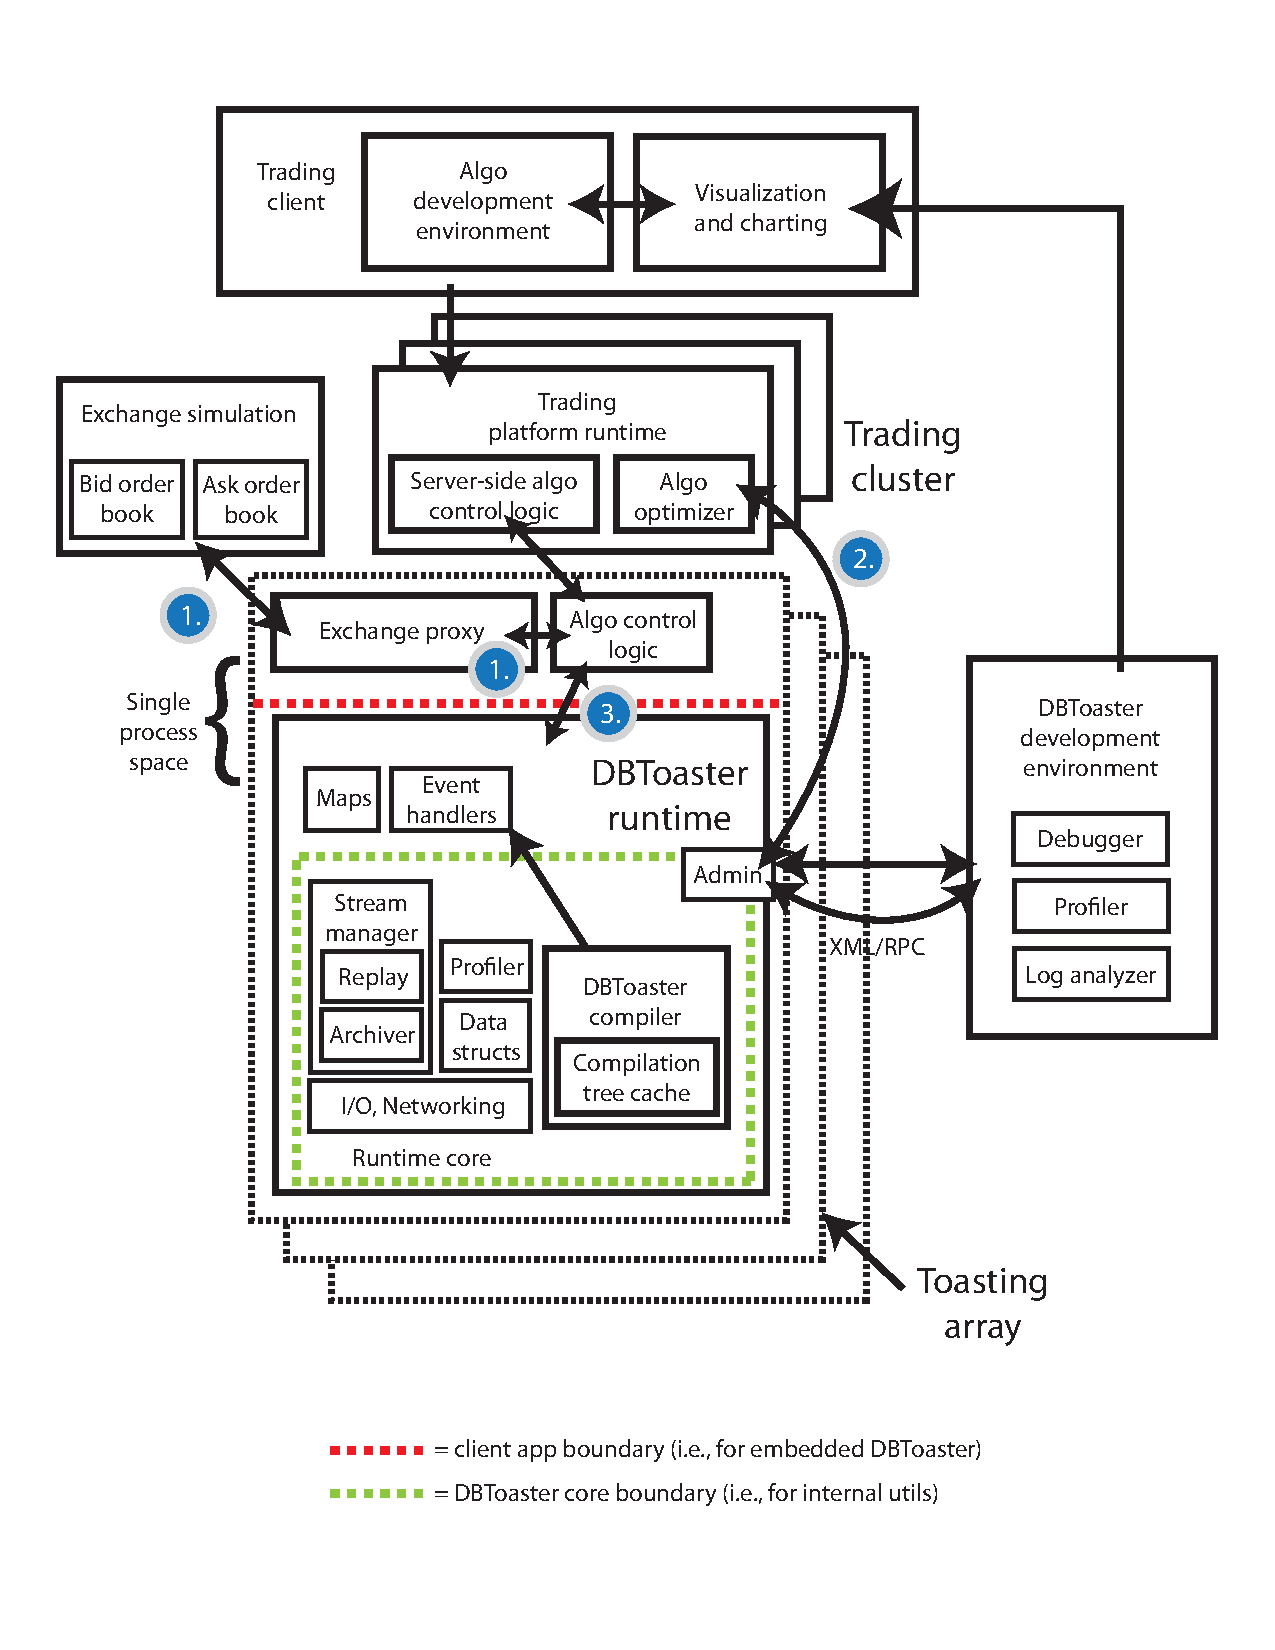
\includegraphics[width=4.50in]{../figures/finapp.pdf}
  \caption{Runtime and AlgoTrader Interactions.}
  \label{TheBigPicture}
\end{figure}

%description of particularities of the system


\section{DBToaster Runtime}

DBToaster Runtime consists of three major components: Compiler, Query Processor and Data Sources Processor. Each of these components also interacts with each other. The complete representation of DBToaster Runtime can be found in figure \ref{DBToasterPic}. 

Each of three components interacts with external environment. Compiler and Query Processor both implement a server to interact with users. Compiler receives SQL queries and data adaptors. Query Processor uses server to distribute query results to users. Data Sources Processor creates user specified clients to receive data from a variety of sources. 

%Compiler receives requests from the client to instantiate a Data Source Reader for receiving data or a SQL query to process data. The created Data Reader is passed to the Data Source Processor and a Query is passed to Query Processor to run on the data. 

\begin{figure}
  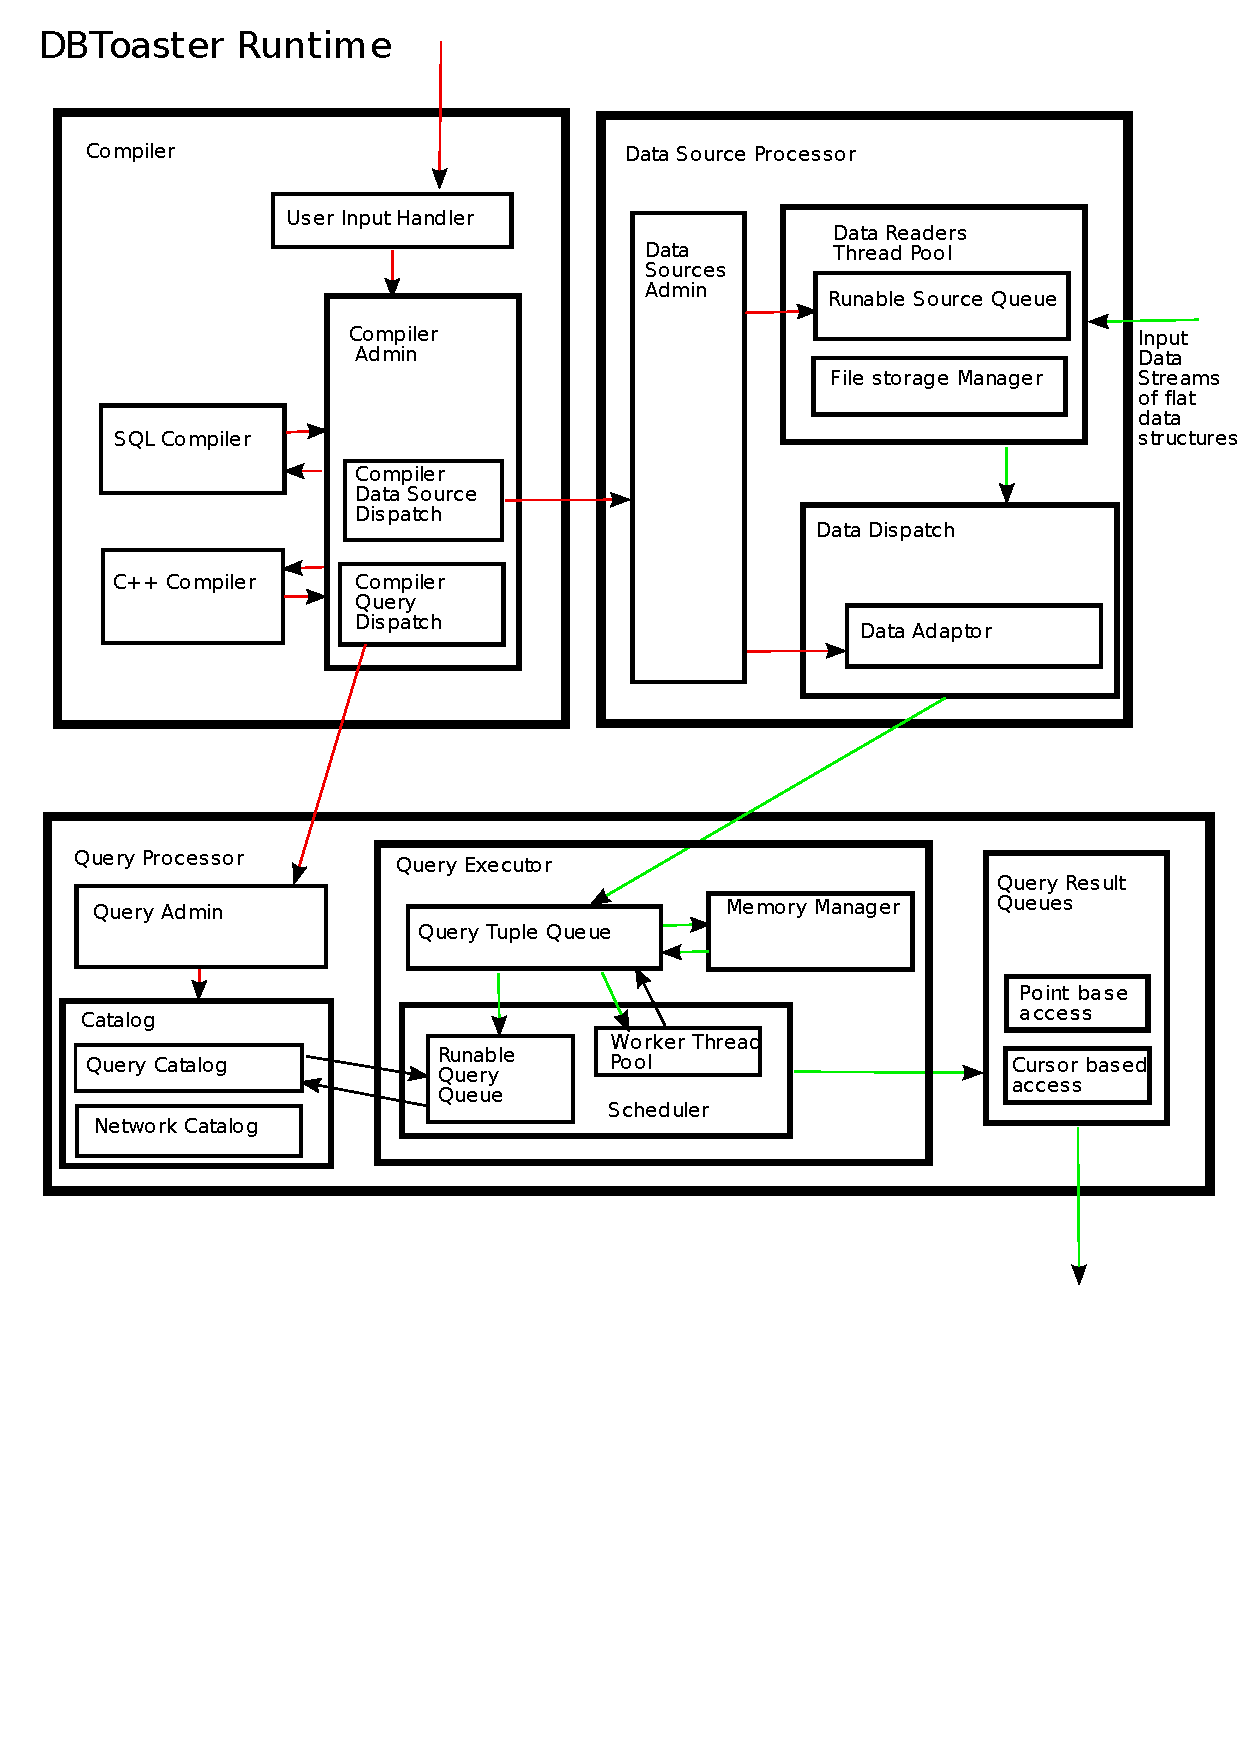
\includegraphics[width=4.50in]{../figures/DBToasterRuntime.pdf}
  \caption{DBToaster Structure.}
  \label{DBToasterPic}
\end{figure}



\subsection{Compiler}

Compiler consists of several components. Its structure can be seen in figure \ref{CompilerPicture}. The main functionality of Compiler is to receive SQL queries and Data Adaptors from users. When they are compiled, Compiler adds them to Sources Processor or Query Processor respectively.

%Two components responsible for compilation are SQL query pre-compiler and C++ code compiler. 

Compiler is an initial point of interaction with the DBToaster Runtime. Once Runtime is up and running users initiate contact by specifying their need to execute a query on some specific set of data sources or a desire to add an update stream. User query and requests to add Data Adaptors are received by User Input Handler. When Input Handler collects all needed informations, it is passed to Compiler Admin. Compiler Admin converts  SQL queries to C++ code and C++ code to binary format. Compiled queries are passed to Query Admin to be added to a list of actively executed queries. Data Source streams (Readers) are added by a user providing a Data Adaptor for each stream. When Data Adaptor code is compiled and user specified Reader is created, both are passed to Data Sources Admin to be added to the list of active Readers. Reader and Adaptor for that Reader form a pair where Reader receives data and Adaptor converts it to a format understandable by Query Executor.

%The Data Adapter is compiled into a binary format and sent to Data Sources Admin to be added to Data Adaptors. 

\begin{figure}
  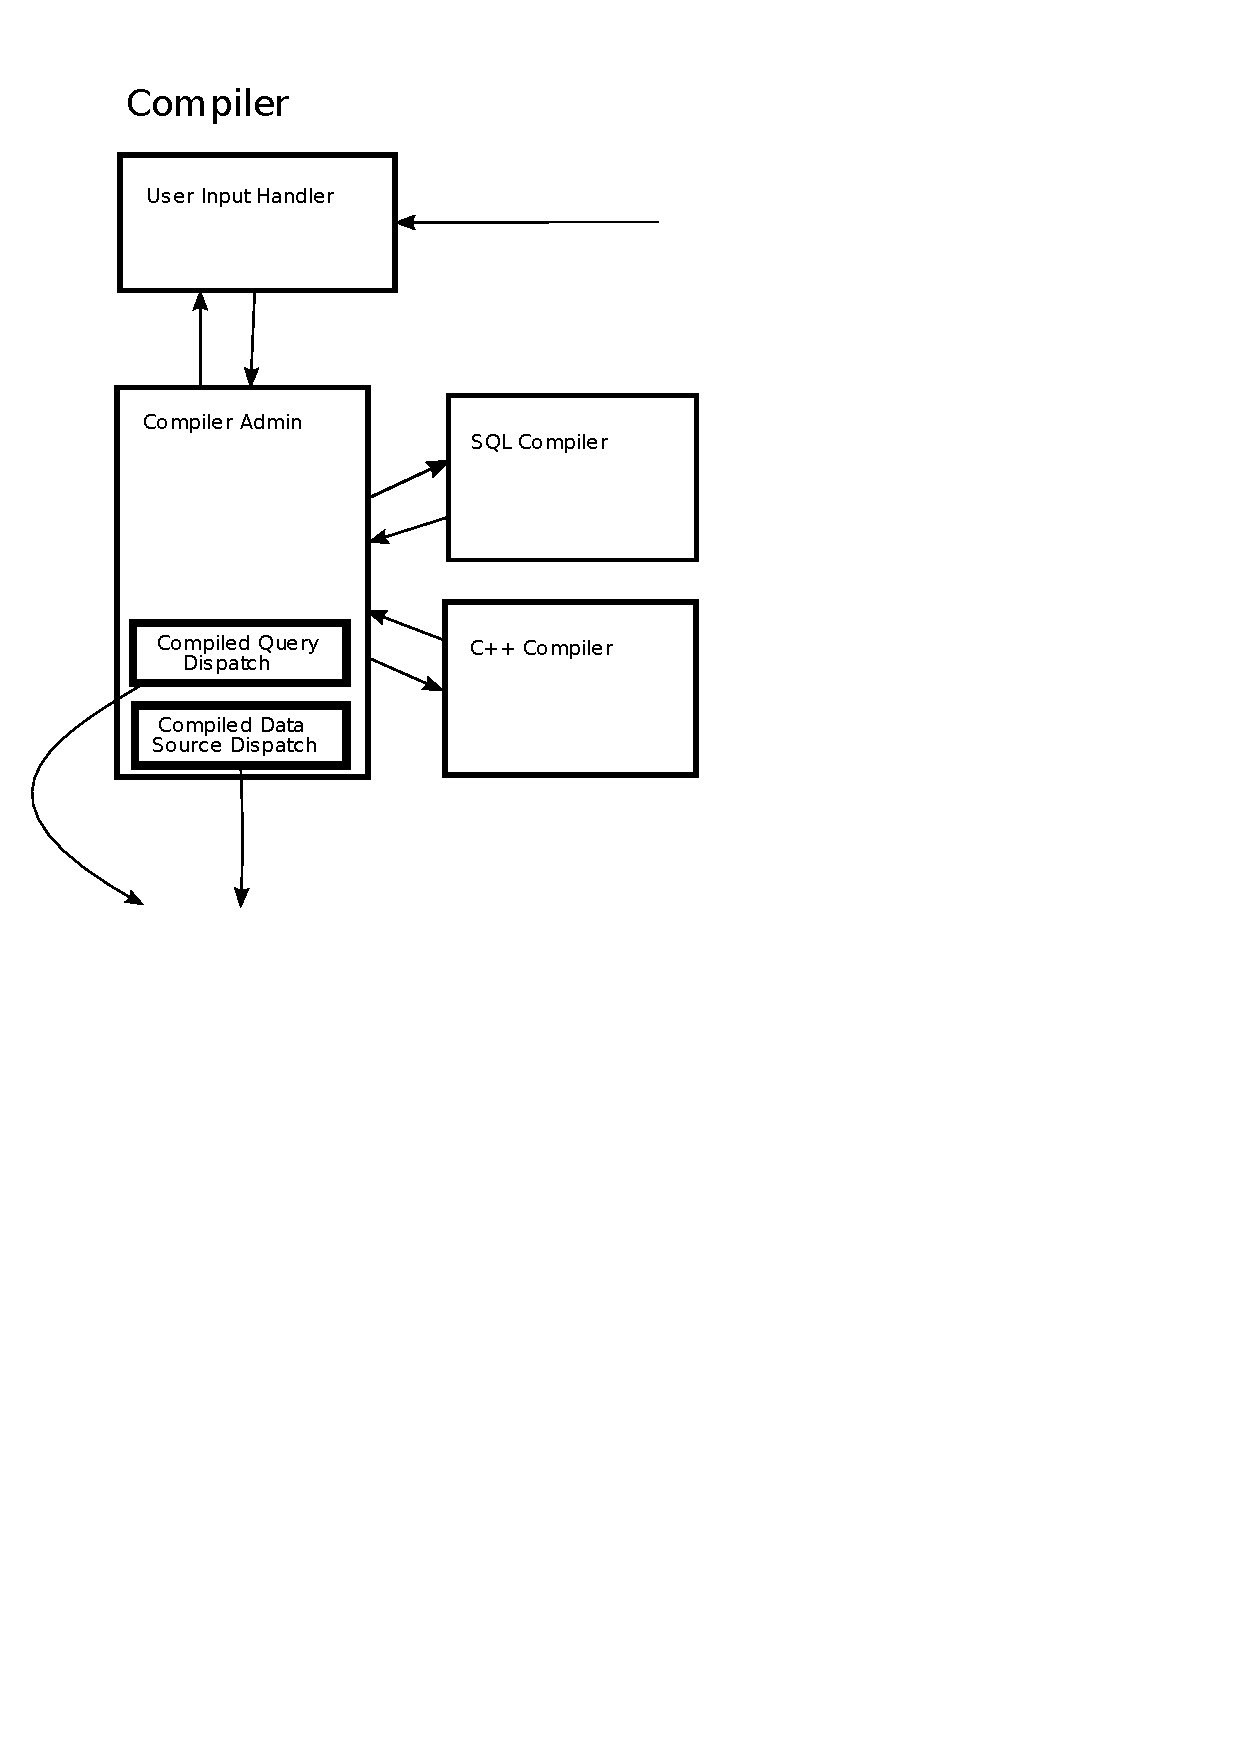
\includegraphics[width=4.50in]{../figures/compiler.pdf}
  \caption{Compiler Structure.}
  \label{CompilerPicture}
\end{figure}

\subsubsection{User Input Handler}
User Input Handler implements a server to handle client requests. Clients connected to Input Handler Server send request types and parameters of that request:
\\
\\
\begin{tabular}{|l|l|}
  \hline
  Type & Parameters \\ \hline
  Query & Query in SQL, list of Data Processor \\ \hline
  Reader & Connection Type, code for Data Adaptor \\ \hline
\end{tabular}
\\
\\
Thus User Input Handler responds to two type of requests one to add a SQL query and another is to add Data Processor.
\\*
Add Query request requires the following information from users:

\begin{itemize}
	\item {\tt AddRequest(type="add query",\\
		 Source="SQL Source File",\\
	     DataReaders="list of Data Adaptors for this query");}
\end{itemize}

\noindent Add Data Stream request is as follows:

\begin{itemize}
	\item {\tt AddRequest(type="add stream", \\
	     AdaptorSource="C++ Adaptor Source file",\\
	     source="IPaddress and port or data input file");}
\end{itemize}

This information is forwarded to Compiler Admin:

\begin{itemize}
	\item {\tt Struct InputRequest( int type, string fileName,\\
	       list<int> informationSources \\
		   list<string> sourceParameters)}
\end{itemize}

User Input Handler serves as an interface for a server. Input Handler and Compiler Admin are currently on the same execution path. In the future if needed Compiler Admin can be separated to run in a different thread with the buffer to store user requests from User Input Handler. 

\subsubsection{Compiler Admin}

Compiler Admin takes source code from User Input Hander, compiles it to executable code and dispatches it to either Data Sources or Query Processor. 
%Once user request is received, Compiler Admin takes over. Depending on the type of the request Admin takes different actions. 

On SQL query request Admin passes SQL query source file to SQL Compiler. SQL compiler returns a file containing C++ implementation of it. This file is passed to C++ compiler. C++ compiler returns a function handle to compiled binary of this query. Finally query handle is passed to Query Admin to be added to a list of executable queries.

On Reader request Admin passes Data Adaptor file to C++ compiler, which returns a function handle to Data Adaptor. Admin creates a Data Source Reader and opens a connection (either a socket or a file). Handle to Data Source together with handle to Data Adaptor is passed to Data Sources Admin.

\noindent Compiler Admin class looks as follows:
\begin{verbatim}
class CompilerAdmin
{
    void RunAdmin(InputRequest);

private:
    cCodeFileName  CompileSQL(string SQL_file_name);
    functionHandle CompileC++(string C++_file_name);
	
    SQLCompiler;
    CCompiler;
    QueryAdmin *;
    DataSourcesAdmin*;
}
\end{verbatim}

Method {\tt RunAdmin(InputRequest)} takes a user request specified by \emph{InputRequest}. Compiler Admin contains SQL Compiler and C++ Compiler. It also contains pointers to Query Admin and Data Sources Admin needed for parameter passing.

\subsubsection{SQL Compiler}

SQL complier takes SQL query from a file and creates an optimized, DBToaster, C++ coded to be added to the runtime. File containing code is returned to the Admin.

\begin{itemize}
	\item {\tt cCodeFileName CompileSQL(SQL file name);}
\end{itemize}

\subsubsection{C++ Compiler}

C++ compiler takes file containing C++ code. It builds binary code, loads it in memory and returns a function handle to it to Admin.

\begin{itemize}
	\item {\tt functionHandle CompileC++(C++ file name);}
\end{itemize}



\subsection{Data Source Processor}

\noindent Data Sources Processor receives updates from various streams. Each stream is handles by a Data Source. Upon receiving an update Data Source passes it so appropriate Data Adaptor. Data Adaptor passes it to appropriate queries. 

Data Sources Admin receives two function handles from Compiler Admin a Data Source and Data Adaptor. 

\begin{itemize}
\item Data Source is inserted into Runable Sources Queue. It receives data from outside streams and forwards received information to data dispatcher.
\item Data Adaptor is inserted into a data dispatcher. Data Adaptor transforms data from Data Source into a format specified by queries.
\end{itemize}

Data Sources Thread Pool stores a set of execution threads and a queue of Runable Data Sources. Each thread 

\begin{itemize}
	\item Picks a Data Source from a queue
	\item Performs a data read 
	\item Forwards read data tuple to Data Dispatcher
\end{itemize}

\noindent Detailed representation of Data Sources Processor can be found in figure \ref{DataSourcePic}.

%where each thread picks a Data Reader and executes a read at a time from one of them. Once read is done the results of the read are forwarded to a Data Structure Dispatch. The Dispatch uses the appropriate Data Adapter to handle the data into a structured format, then the structured data is forwarded to Query Processor, in particular to the Query Tuple Queue. The more pictorial description can be found in figure \ref{DataSourcePic}.

% processing consists of the list of list of stream points. Each point is given by the user and signifies a way for a DBToaster to connect with the input stream of some process which dispatches data to the DBToaster. Each Stream Point is written by the user and user can fully specify how the data should be received and processed. Stream point is responsible for sending data to the Data Dispatch unite in a pre-specified format. The structure for data source processing can be found in figure 

\begin{figure}
  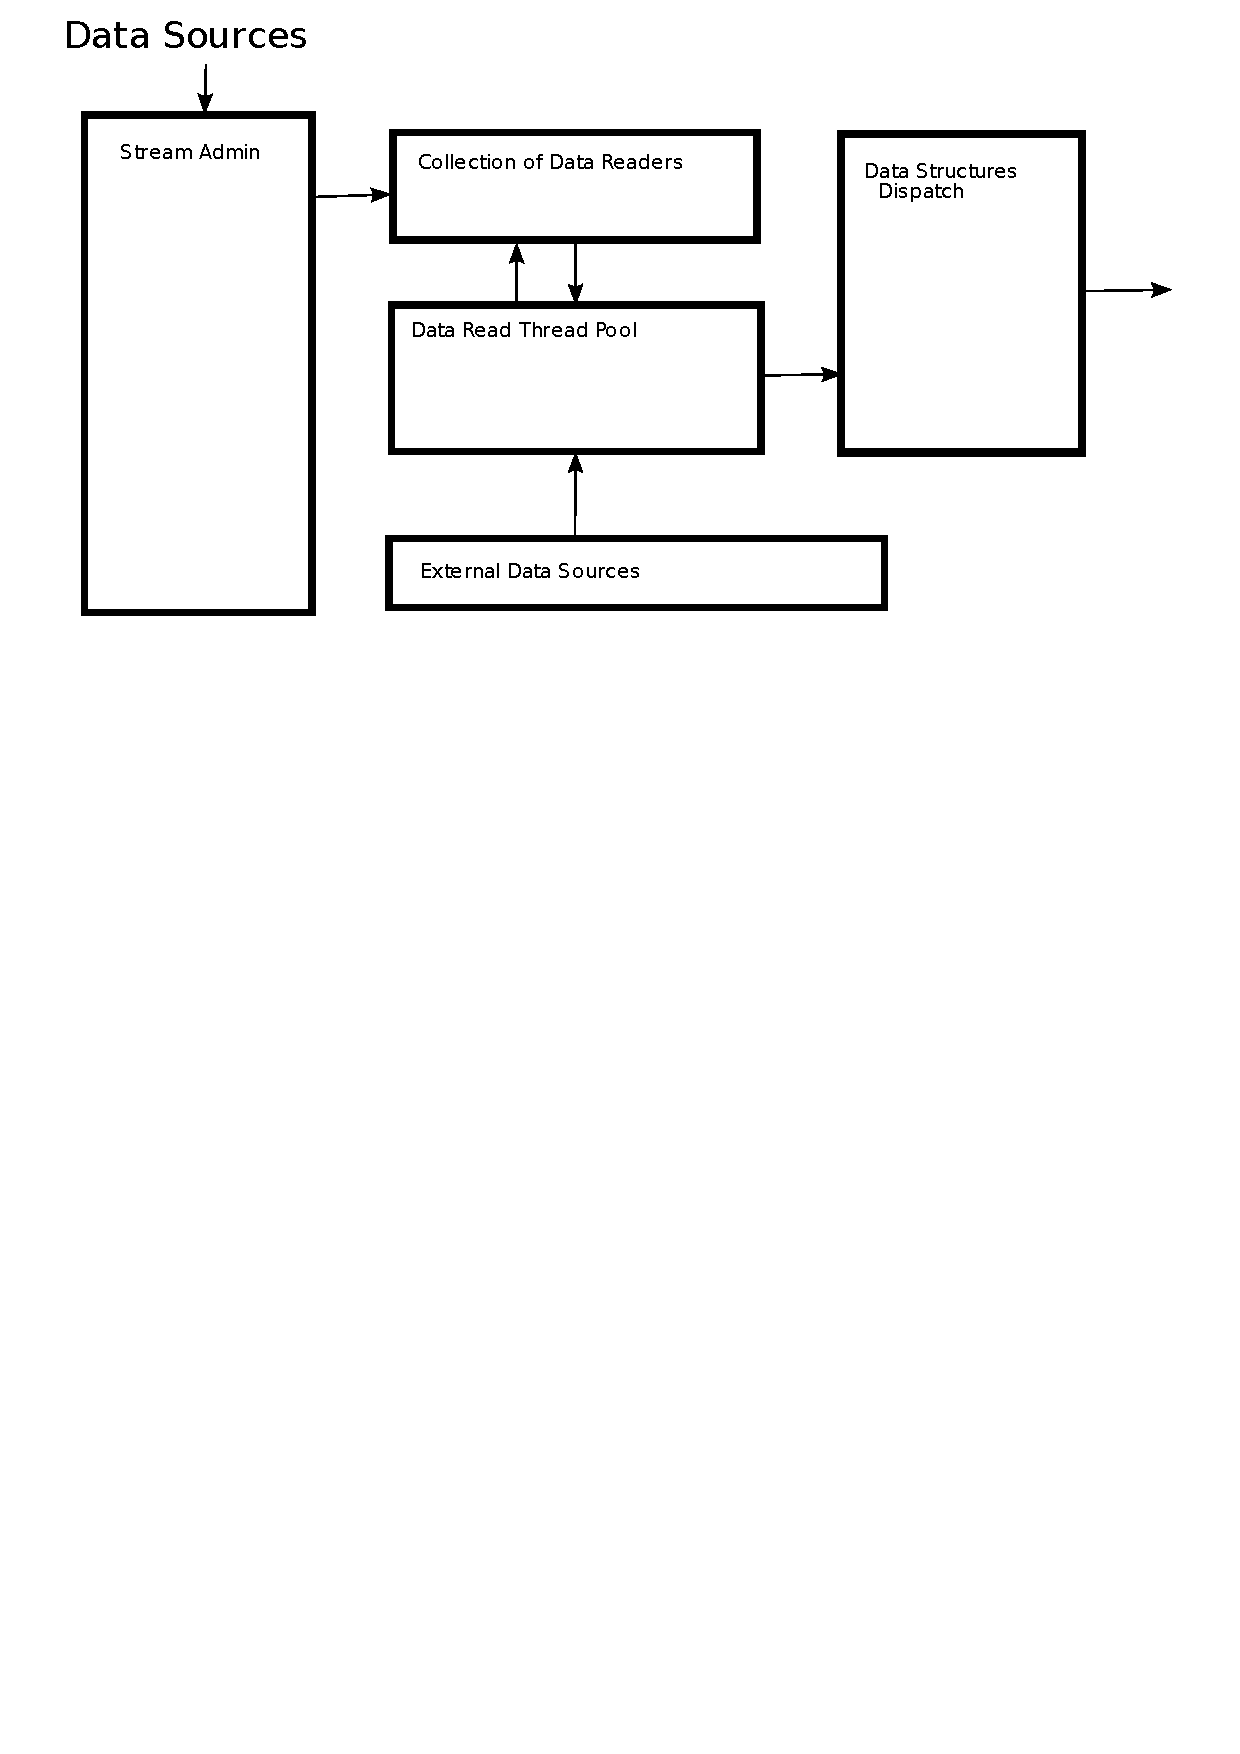
\includegraphics[width=5.00in]{../figures/DataSources.pdf}
  \caption{Data Sources Management.}
  \label{DataSourcePic}
\end{figure}

\subsubsection{Data Sources Admin}

Data Sources Admin provides an interface for adding new Data Sources. Each Data Source is paired up with a Data Adaptor. The later conversts raw data tuples to format understood by query.

Another reason for Data Sources Admin is to provide a level of abstraction since calls for Data Source and Data Adaptor additions will be executed in the compiler execution path. 

\begin{verbatim}
class DataSourcesAdmin
{
    DataSourcesAdmin(InputBufferInterface*);
    addDataSource(sourceID, SourceReader, DataAdaptor);

	DataDispatcher;
    DataSourcesManager;
	InputBufferInterface*;

}
\end{verbatim}
 
\noindent Data Source Admin is also responsible for handling Data Dispatcher and Data Sources Manager.


%Data Sources Admin receives two function handles one to a data Reader and another one for a Data Adaptor from a Compiler. First Admin locks Data Adaptors and inserts a new Data Adaptor. Then Admin locks Data Readers Queue  and a handle is inserted. Each Data Readers handle implements a method \emph{readNext()} for reading data from some data source (typically a socket or a file).

%\begin{itemize}
%	\item {\tt rawDataTuple getNext(); // user defined function - provided}
%\end{itemize}

%\noindent The {\tt rawDataTuple} is a pair {\tt <size, bit-string>}.

%The Reader extracts the informations from either a file or a socket. Reader's communication with the outside world is in a standard format. On a read request, Reader first reads a header containing the information about the message followed by the message itself. For now we assume that a header is an integer containing the number of byte to be read. Once the read is completed the size and message are forwarded to Data Structures Dispatch.

%\noindent Data Sources Admin class contains the following:



\subsubsection{Data Sources Manager}

Data Sources Manager contains a list of identical threads. Each thread is responsible for getting a Data Source from queue of Data Sources, reading next update \emph{readNext()} message, and sending this {\tt rawDataTuple} message to Data Dispatch together with Dat Source ID.

Data Sources Manager is structured as follows:
\begin{verbatim}
class DataReadersPool
{
	void Run();
	
    list<thread>            runningThreads;
    DataReadersQueue        sources;
    DataDispatch *          outputBuffer;
}
\end{verbatim}

\noindent It contains a Data Readers Queue:

\begin{verbatim}
class DataReadersQueue
{
	functionHandle  getNextReader();
	void            putNextReader(functionHandle);
	
    queue<functionHandle>  sources;
}
\end{verbatim}

\noindent and a pointer to Data Dispatcher.

\subsubsection{Data Dispatcher}

Data Dispatcher receives ID identifying a Data Source and a message read by that Source. 

\begin{itemize}
	\item {\tt dispatchNext(readerID, rawDataTuple);}
\end{itemize}

Based on Data Source ID Dispatcher calls an appropriate Data Adaptor to convert incoming {\tt rawDataTuple} message into a structure messages understood by queries. Structured tuple is then sent to an appropriate set of queues in the Input Buffer. {\tt structuredTuple} is a pair {\tt <size, bit-sequence>} such where bit sequence can be processed by queries. 

\begin{verbatim}
class DataDispatcher
{
	
    void dispatchNext(readerID, rawDataTuple);

private:
    void sendData();
	
    DataAdaptors;
    InputBuffer*;
}
\end{verbatim}

\noindent Data Adaptors is a map enabling access to appropriate Data Adaptor for a given Data Source.

\begin{verbatim}
class DataAdaptors
{
public:
    functionHandle  getAdaptor(sourceID);
    void            addAdaptor(sourceID, functionHandle);

privare:
    map<sourceID, functionHandle>;
	
}
\end{verbatim}

\subsection{Query Processor}

The bulk work of Query Processor is done in Query Executor with a set of Query Threads. Each thread picks a query-datum pair from a pool of available pairs and processes it. As data comes in from Data Dispatcher, it is sent to the appropriate set of queries. When query receives a datum it becomes available for execution. The structure of query processor can be found in figure \ref{QueryProcessingPic}.

\begin{figure}
  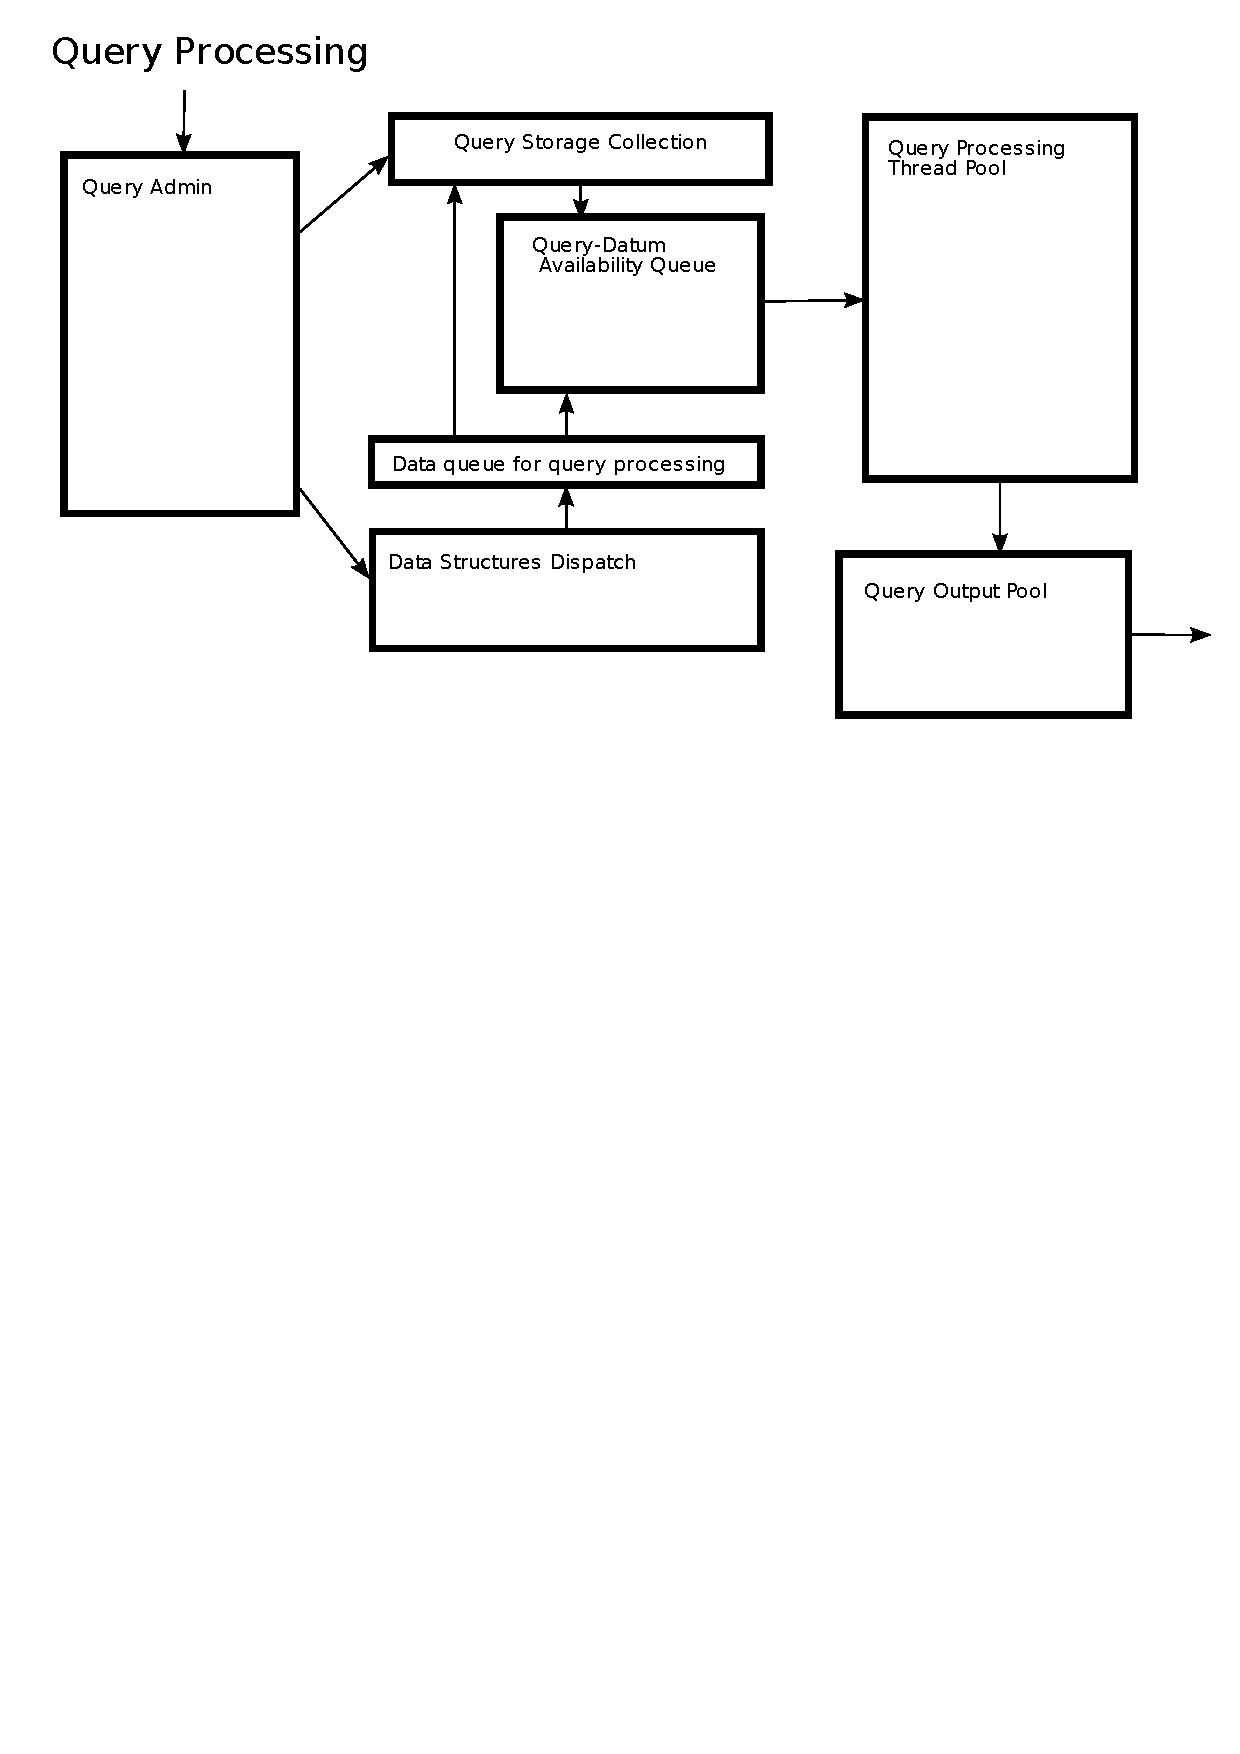
\includegraphics[width=5.00in]{../figures/QueryProcessing.pdf}
  \caption{Query Processing Management.}
  \label{QueryProcessingPic}
\end{figure}

\subsubsection{Query Admin}

Query Admin receives a function handle to a query. It also receives a list of Data Source IDs which provide data for that query. When Query handle is received, Admin locks Query Catalog and inserts query handle there. After that Query Results Queue is locked and updated to create an output queues for just inserted query. Finally Admin locks Query Tuple Queue and inserts and additional queue for data associated with inserted query. 

Query Catalog is a map containing query ID and a handler for that query. 

Query Admin class looks as follows
\begin{verbatim}
class QueryAdmin
{
    addQuery(queryID, functionHandle, list<int> ReadersID);

	queryCatalog;
	networkCatalog;
	QueryTupleQueue*;
	
}
\end{verbatim}

\subsubsection{Query Executor}

Query Executor consists of two inter dependent components: Input Buffer and Scheduler. Input Buffer stores data needed for query execution. Scheduler contains a set of threads. Each thread runs one query at a time one update tuple from Input Buffer. \emph{InputBufferInterface} and \emph{SchedulerInterface} are two classes providing interface for \emph{InputBuffer} and \emph{Scheduler}. 

\paragraph{Input Buffer}

Input Buffer provides seamless access to the data and storage. It contains a queue per data source. Each query needs to register with queue to access data from it. Input Buffer receives a new tuple from Data Dispatch with an ID of its data Source (in a format {\tt structuredTuple}), the new tuple is inserted into appropriate queue. If a tuple insert causes query to become available Scheduler is notified to add such a query for processing. If a query is already runnable, a tuple is just inserted into appropriate queue without any action.

\noindent \emph{InputBufferInterface} has the following structure:

\begin{verbatim}
class InputBufferInterface
{
    void                  addTuple(int sourceID, void * structuredTuple);
    void *                getTuples(int queryID);
    void                  addQuery(int queryID, int sourceID);
    void                  removeQuery(int queryID);
    void                  hasNext(int queryID);
    void                  removeTuples(int queryID);
	
}
\end{verbatim}

\noindent Input Buffer class has the following structure:

\begin{verbatim}
class InputBuffer
{
	InputBuffer(MemoryManager* Jim);
    void             addTuple(int sourceID, void * structuredTuple);
    void *           getTuples(int queryID);
    void             addQuery(int queryID, int sourceID);
    void             removeQuery(int queryID);
    void             hasNext(int queryID);
    void             removeTuples(int queryID);
    void             addScheduler(SchedulerInterface* sch);

	MemoryManager*                     Jim;
	Scheduler*                         schedulingQueue;
	map<sourceID, list<TupleQueue*> >  sourceAccess;
	map<queryID, list<TupleQueue*> >   queryAccess;
	map<sourceID, list<queryID> >      availableQueries;
	
}
\end{verbatim}

\noindent Here we refer to {\tt queryID} as an ID of a query, which needs data from a particular data source. This ID is created in Query Catalog. Its purpose is to make a direct link between a query and a source. It hides details of dealing with several sources for each query inside Scheduler.

Interface function {\tt addTuple(sourceID, structuredTuple)} is called by the Data Dispatch to add a new data item. Functions {\tt getTuple(queryID)},{\tt hasNext(queryID)} and{\tt removeTuples(queryID)} are required to extract tuples available for the query to be executed as well as for cleaning up queues. Functions {\tt addQuery(int queryID, int sourceID)} and {\tt removeQuery(queryID)} are needed by Query Admin to insert or remove a new queries. 

To enable this functionality we need to consider concurrency and efficiency. 

\subparagraph{Concurrency:} Each queue can be accessed by several queries. Also each queue has only one data source associated with it. The queue is locked on insertion and deletion form Data Source. Data reads are enabled to all queries simultaneously. \emph{SharedTupleQueue} provides this controls internally for each queue. Since there is no race between different queues there is also no need to create concurrency between them.

\subparagraph{Efficiency:} The main inefficiency comes form a fact that data from one data source needs to be accessed by several queries. If we adopt a simple model (case A), each query has its own set of queues for each of required sources. Here we have inefficiency of coping data to each such queue. The benefit of such model is its simplicity of implementation and use. Also no need for concurrency mechanisms. Another model (case B) is to have only one queue for each data source. In this case each queue will need to keep track of which query requires what data item from this queue. Data deletion becomes complicated. The benefit of this method is simpler storage method and memory management. Both approaches can be supported. We can hide all details into the implementation of queue and Input Buffer. By requiring the following specification:

\noindent Case A:
\begin{verbatim}
class QueryTupleQueue
{
    QueryTupleQueue(MemoryManager*);
	
	void              addTuple(structuredTuple);
	void *            getTuples();
	bool              isEmpty();

	queue<StructuredTuple>   tuples;
}
\end{verbatim}

\noindent Case B:
\begin{verbatim}
class SharedTupleQueue
{
    SharedTupleQueue(queryID, MemoryManager*);

	TupleQueue*       join(queryID);
	void              removeQuery(queryID);
	
	void              addTuple(structuredTuple);
	structuredTuple   getTuples(queryID);
	bool              isEmpty(queryID);
	void              removeTuples(queryID);
	
	map<queryID, pointerToPositionInQueue>     nextTuple;
	queue<SharedTuple>                         datum;
	MemoryManager*                             memMan;
}
\end{verbatim}

\begin{verbatim}
struct SharedTuple
{
    int              beenAccessed;
    StructuredTuple*  datum;
}
\end{verbatim}

In current implementation we decided to adopt Case B due to memory savings and efficiency of data copying copying.

When a new query is inserted into Query Admin, Input Buffer is called with {\tt addQuery(queryID, int sourceID)} for each data source (remember that queryID is an ID indicating query source connection and is mapped to a real query in Query Catalog). If a source is not present (we can find it though {\tt map<sourceID, list<TupleQuery*> >}) we create a new Tuple Queue. If it is present, we call {\tt join(queryID)}. {\tt join(queryID)} in case A will create a new TupleQueue and return a pointer to it. In case B, it will return a pointer to this queue and change internal structure to accommodate a new query. ({\tt removeQuery(queryID)} is a reverse. It is either remove a queue or changes internal representation). New tuples are added by the call of {\tt addTuple(sourceID, structuredTuple)} in \emph{InputBuffer} from Data Dispatcher.

\subparagraph{Memory Manager} facilitates storage of data tuples by pre-allocating a number of pages. Memory Manager creates an interface for allocating and deallocating space for data by allocating a set of new page and deallocating unused pages. 

\begin{verbatim}
class MemoryManager
{
    void * getPage();
	void   returnPage();
}
\end{verbatim}

\noindent To ease the management of page memory class Pages Manager is created. It keeps track of all relevant information needed to allocate space for new tuples.

\begin{verbatim}
class PagesManager
{
    PagesManager(MemoryManager*);
    void * getSpace(int* size);
    void   free(void* position, int* size);
    
}
\end{verbatim}

\paragraph{Scheduler}

Scheduler's job is to execute a query on an appropriate data tuple. This goal is achieved by creating a set of identical threads for executing queries. Each thread is responsible for picking up a query from Runable Query Queue. Then thread runs a query on data tuple from Input Buffer. Results are put into a Query Results Queue. Results are accessed by users upon request.

The execution flow within each thread is as follows:

\begin{verbatim}
get a queryID from RunableQueryQueue;
get data: a set of data tuples from Input Buffer;
get a query handle from QueryCatalog;

run Query on data;

release data in InputBuffer;

if more data for this query is available
	put query onto RunableQueryQueue;

put results to QueryResultsQueue;
Repeat...

\end{verbatim}

Scheduler class contains the following:

\begin{verbatim}
class Scheduler
{
	Scheduler(QueryCatalog*);
    void       Run();
    void       addRunableQuery(querySourceID);

    RunableQueryQueue   availableQueries;
    list<thread>        executionThreads;
    InputBuffer *       readyData;
	QueryCatalog*       queryHandles;
	
}
\end{verbatim}

Function {\tt addRunableQuery(querySourceID)} is used by Input Buffer to check if current query is available for running. If query is not available it is added to Runnable Queries.

\noindent With RunnableQueryQueue as follows:

\begin{verbatim}
class RunnableQueryQueue
{
    
    queryID        nextQuery();
    void           addQuery(queryID);
    void           removeQuery(queryID);
    bool           isActive(queryID);

    queue<queryID>    readyQueries;
	
}
\end{verbatim}


\subsubsection{Query Results Queue}

Query Results Queue implements a server, where each client upon connection indicates a set of queries they are interested in.

\begin{itemize}
	\item {\tt userDataStructuresDispatch(userID, Query ID list);}
\end{itemize}

\noindent Server creates a map of query IDs to query results for each client. When a query produces an output, it is sent to Query Result Queues. There query results are dispatched to appropriate queues.

\begin{itemize}
	\item {\tt queryDataStructuresDispatch(queryID, queryMap);}
\end{itemize}

\noindent When a client needs a new piece of information it sends a request to server with query ID and number of tuples needed.  Server returns  results of that query. 

Query Result Queues implements two ways to access data. In the first one a user asks for a complete query result. In the second one user asks for a cursor to query results and is capable to iterate over results.

Query Result Queue class is:

\begin{verbatim}
class SchedulingQueue
{
    
	map<queryID, queryResult>
	
	getFullQueryResult(clientID, queryID);
	
	startCursorResult(clientID, queryID);
	
}
\end{verbatim}








\section{AlgoTrader}

AlgoTrader is an application that applies DBToaster Runtime to a domain of Stock Exchange and Algorithmic Trading. It consists of two parts: an automatic Stock Trading Simulator and a platform for development and execution of Automatic Stock Trading Algorithms. The purpose of AlgoTrader is to demonstrate the potential of DBToaster Runtime to process time critical, expressive queries over streaming data. To demonstrate the potential of Runtime two components are needed: a source(s) of update stream and an application(s), which runs queries over it. Exchange Server Simulator provides a source of continuous stock transactions between interested parties. AlgoEngine implements a set of trading strategies. Each strategy utilizes results of a query over the data from Exchange Server Simulator to make a decision about purchase/sell of stocks. Queries are processed and executed by DBToaster Runtime.
  

\subsection{Exchange Server Simulator}
Exchange Server Simulator (ESS) is designed to reproduce the behavior of Electronic Communication Networks (ECN). ECN facilitates stock exchanges between different parties connected to the network. Each ECN provides certain data to its subscribers. For now we limit ourselves to complete knowledge about changes in stock order books. Order books for a stock contains all sell (ask) and buy (bid) request for each stock. This data is distributed to all subscribers as a constant stream of updates to order books. Current implementation of Exchange Server Simulator works with only one stock (for now). 

Each Order Book consists of an Asks Book and Bids Book. Asks Book contains sell requests, Bids Book - buy requests. Each ask/bid request is transmitted to all subscribers. If two requests are matched the results of such a match are transmitted as well. 

Main difference between a real ECN and a Simulator, is simulator's ability to replay the exchanges made at some earlier date and incorporate exchanges made by trading algorithms into this stream. 

We implemented ESS to support two types of clients: readers and writers. Reader clients constantly listen to a stream of messages without placing any orders. Writer clients only place orders and interact with Simulator to get the information about just placed order (like order ID). The detailed implementation of ESS is as follows.

\subsubsection{Exchange Server}
ExchangeServer creates a local host server on a given port and handles all incoming client connections. Each connected client is processed in its own thread (ExchangeThread). ExchangeServer also creates a data client (DataThread). This client is responsible for reading historical data from a file, connecting to a server and transmitting data to server. Server also creates structure for storing order book information. It is shared by all clients.

\noindent The basic structure of Exchange Server is as follows:
\begin{verbatim}
open(Server_Socket);
SynchronizedBooks DataBook;
DataThread historical_data(inputDataFile.cvs);
historical_data.run();

while (Server_socket.listen())
{
    get(client);
    run(client, DataBook);
}
\end{verbatim}


\subsubsection{Exchange Thread}
When a client connects to ESS, ExchangesThread is created to handle client needs. All ExchangesThreads share order book storage structure: \emph{SynchronizedBooks}. They also share a list of all connected clients.

\noindent The communication protocol between a client and a server is as follows: 

\noindent The first message a server expects form a thread is a client type.

\begin{tabular}{|l|l|}
  \hline
  \multicolumn{2}{|c|}{Client type} \\
  \hline
  0 & Writer\\ \hline
  1 & Reader \\
  \hline
\end{tabular}
\\
\\
\emph{Writer} clients are designed to send data and receive messages only as a response to their transactions. \emph{Reader} clients receive all ongoing transactions but do not to send messages themselves.

Communication messages  are in pre-specified format:

\begin{verbatim}
long time;
int  order_id;
int  brokerage_id;
char action;
int  volume;
int  price;
\end{verbatim}

Where \emph{time} indicates the time when requests arrived to the server, \emph{order\_id} a unique identifier for each order given by ESS, \emph{brokerage\_id} ID identifying company, which placed an order, \emph{action} one of several actions (buy, sell, cancel) described below, \emph{price} and \emph{volume} are price and amount of stocks to be bought/sold. 

\noindent Several action can possibly occur:

\begin{tabular}{|l|l|}
  \hline
  Request & Action \\ \hline
  'B' & buy request, check ask book for match, if none add it to bid book \\ \hline
  'S' & sell request, check bid book for match, if none add it to ask book \\ \hline
  'D' & delete request for an appropriate book if one exists \\ \hline
  'X' & cancel order remove trade request from appropriate book\\ \hline
  'E' & change request, generated by server \\ \hline
  'F' & order fulfilled, generated by server \\
  \hline
\end{tabular}
\\
\\
\noindent 'B', 'S' and 'D' actions can come from any of the clients (as a buy or sell stocks request or delete request). Actions 'E', 'F' and 'X' are generated by server as a result of a partial match, match or delete request. 

Each transaction and its consequences are announced to all Reader clients as well as to Writer client, which initiated a transaction. 

The basic operation of each Exchange Thread is:

\begin{verbatim}
while (listen(request)){
	messages=DataBook.update(request);
	foreach(Reader)
	 send(messages);
}
\end{verbatim}

% the first  message showing an interest in exchange ExchangesThread checks if there is an appropriate match in the data structures (i.e. if some one wants to sell some amount of stocks the thread will look if someone wants to buy stocks at the given price), if so the match is executed if not the request is stored in the data structures. The results and the transaction are announced to all the connected clients. 

\subsubsection{Synchronized Books}
SynchronizedBooks is a shared data structure for storage of order books information. It is shared between all clients. Each client can add/remove/modify it based on client's requests. SynchronizedBooks contains two SortedBooks representing Asks/Bids Books. SortedBook is a structure that has properties of a sorted set and a hashtable. (Data is sorted by data values and can be accessed using keys).

When a sell/buy request is inserted into SynchronizedBooks, it tries to find a matching buy/sell request. If a matching request is found an update message is generated in addition to sell/buy message. Update message contains information about the fact that one or both of the orders are partially/fully satisfied. Update message can be of the form:


\begin{tabular}{|l|l|}
  \hline
  Action & Meaning \\ \hline
  'E' & order number, update amount \\ \hline
  'F' & order was executed in full \\

  \hline
\end{tabular}
\\
\\
SynchronizedBooks utilizes Order\_tuple to store each individual bid/ask request in SortedBooks. Stream\_tuple is used to generate a communication message to be sent to clients.


\subsubsection{Historical Data}

ExchangeServer is capable of using historical data flow from stock trades between real clients in addition to transactions provided by Writer clients. ESS uses DataThread to extract historical data from a file and transmit it to server. DataThread can be started at any point during the execution by a server (for example, once there is a client connected to server). DataThread reads historical trace file in a .cvs format and transmits each message to server as if it was a real request. DataThread does not distinguish between client and server historical actions and transmit all of them as if they were requests made by some client. ExchangeThread distinguishes orders coming from historical data and from live clients by the message's data. Historical data contains order ID and timestamps for all orders. Writer clients have 0 in those fields (except for delete).  


\subsection{Algorithms Engine}

Algorithms Engine is an application designed to emulate actions of a hedge fund. It implements a set of trading algorithms. Each trading algorithm runs a query over data produced by Exchange Server Simulator. Based on this information an algorithm makes a decision whether to buy or sell stocks. Those requests go directly to ESS. 

Algorithms Engine has two connections to ESS. First connection is a writer client. It sends ask/bid requests to ESS. The second connection is a reader client to monitor the results of exchanges. The second connection notifies Algorithms Engine when and if ask/bid request have been executed. 

There are two concurrent execution paths inside Algorithms Engine. First path creates a reader client to ESS and starts listening to the update stream. Each order in a stream is compared to a set of internal order requests. If an incoming data is about one of the internal requests, this request is modified and appropriate statistics are changed. The second path creates one writer connection to ESS and a client connection to DBToaster Runtime. This path starts by initiating all trading algorithms. Each  trading algorithm runs (or uses results of) a query over data produced by ESS. These queries are executed by Runtime. Results of each query are used by Algorithms Engine. When data is available, trading algorithms use it to determine whether to place ask/bid order. This process repeats continuously. 

%Algorithm Engine code developed by the end users. The code makes use of DBToaster Runtime to query the continuous data from input streams specified by the users. The query results are then processed by user defined algorithms to achieve their goals. 

%In our example Algorithmic Engine creates and runs a set of monitoring queries for the stock trading depending on the results of the queries and the internal mechanics - algorithms decide to buy or sell stocks on a NASDAQ Trading Exchange Simulator.

\subsubsection{Algorithms Engine Class}

AlgorithmsEngine class contains all trading algorithms, connections to ESS and a connection to DBToaster Runtime. On initiation it starts Reader connection to ESS. A trading algorithm can be added at any time during execution. 

\begin{verbatim}
class AlgorithmsEngine
{
    AlgorithmsEngine();
    void runAlgos();
    void addAlgo(AlgoInterface * algo);

private:
    void getData();
    
    list<AlgoInterface*> my_algos;
    DataCollection       data;
    OrderManager         manager;
	
}
\end{verbatim}

DataCollection is an interface to DBToaster Runtime. It contains query results. OrderManager contains statistics for each algorithm and order requests from all algorithms. 

The execution cycle of \emph{runAlgos()} is

\begin{verbatim}
void runAlgos()
{
    getData();
    
    foreach algo in my_algos
        requests=algo->run(requests);
    
    manager.handle(requests);
}
\end{verbatim}

Where \emph{requests} is a set of order requests generated by algorithms.

%Algorithmic Engine interacts with environment in three different ways. First of all the Engine needs to receive  the information from from DBToaster runtime. This interaction is unavoidable since the Engine needs the results of the queries. Another interaction which needs to be added is the way to specify the information stream received by a DBToaster runtime. This information needs to be passed the the Runtime in the form of c++ code for the Runtime to compile. Another optional source of interaction is infulencing the enviroment. In our example is the Engine's capability to add/remove stock requests from the Exchange Server. 

\subsubsection{Order Manager}
OrderManager is an interface with ESS. 

\begin{verbatim}
class OrderManager
{
    void sendOrders(function handler, deque<AlgoMessages*> messages);
    void startReading(boost::asio::io_service& io_service)
    void processOrder(DataTuple & tuple);
    
private:
    WriterConnection *             writer;
    WriterConnection *             reader;

    ptr_map<LocalID, DataTuple>   dataOrders;
    ptr_map<OrderID, LocalID>     orderIDtoLocalId;
    ptr_map<LocalID, DataTuple>   executedOrders;
}
\end{verbatim}

Order Manager has two connections to ESS: a writer and a reader clients. Each of them runs in different thread. Reader client is invoked by \emph{startReading} function. It creates a loop where \emph{processOrder} is called repeatedly. Writer client is invoked by \emph{sendOrder} function. It gets a list of order requests form trading algorithms, adds them to \emph{dataOrders} list and sends them to ESS. \emph{processOrder} function in turn checks \emph{dataOrders} whether it contains an order with the same order ID as incoming message \emph{tuple}. If it does the update to \emph{dataOrders} is made and changes in statistics for appropriate algorithm.

\emph{executedOrder} stores all completed requests. \emph{orderIDtoLocalId} is a map from Server's identifier for each order to internal identifier used by Order Manager for each order.


\subsubsection{Data Collection}
DataCollection class provides high level interface to ESS. It contains a \emph{ToasterConnection}. 

\begin{verbatim}
class DataCollection
{
    void ReadSOBI();
    void update();
    ToasterConnection toaster.
}
\end{verbatim}

Toaster Connection is a thrift client to DBToaster Runtime. It collects results of queries from Runtime. 

Data Collections also contains a number of read and update functions to collect and extract needed data from query results.

%\subsubsection{Data Stream}

%There are two interactions with outside systems needed to be implemented by the user. The first interaction is with DBToaster. A system needs to pull information from the DBToaster runtime. \emph{TODO description of the the pulling mechanism}.

%Another interaction, which needs to be passed to the DBToaster Runtime, is a way for Runtime to access the data streams relevant to the Engine and over which the queries needed to be post. This information is specified as a C++ code which is sent for the compilation to the Runtime to be added to the system.

%\subsubsection{External Influence}

%If the Engine implements interactive process, which needs to access outside processes or interact (influence) them then this is interactivity needs also to be added. In our example Algorithmic Engine can buy and sell stock on our Exchange Simulation Server. Thus acting like one of the clients of the server. \emph{TODO describe the system in more details}

\subsubsection{Algorithms}

Algorithms are the most interesting part of Algorithms Engine and are a driving force for DBToaster Runtime. Each Algorithms makes a decision about buying or selling stocks based on information received from ESS. Relevant information for each algorithm can be extracted by running a query over Order Books of ESS. DBToaster Runtime provides the functionality to do so. 

Currently there is a set of algorithms implemented by Algorithms Engine. 

\paragraph{Simple SOBI}

Static Order Book Imbalance (SOBI) is a strategy of comparing the difference between last known stock price and volume-weighted average price (vwap) of stock in each order book. For example, a much greater difference between last price and vwap of an ask book to that of bid price indicates that sellers do not support current price and that price has a great chance of rising. (The reverse works for bids.)

Simple SOBI strategy looks at this imbalance and when one value is four times greater than another, simple SOBI buys/sells a fixed number of stocks at a current price. (Four times greater is completely arbitrary number)

\paragraph{Volatile SOBI}

Volatile SOBI is a derivation of simple SOBI. It additionally takes into account information about price's standard deviation. The strategy buys/sells stocks when the difference between vwap and last price is greater than standard deviation.

\paragraph{Timed SOBI}

Timed SOBI is a strategy similar to Simple SOBI. It looks at an average timestamp for the top orders in each order book. A shift to older values of time stamps indicates lessened support of the current price in this order book. Appropriate buy or sell order is generated for a fixed number of shares and at a current price. 

\paragraph{Market Players}
 

This strategy creates a query over both Order Books. This query looks for all traders, which try to sell and buys stocks at the same time. In particular it looks for cases where a trader wants to sell small amount of stocks at a price a little bit higher than a current price. And the same trader wants to buy a large amount of stocks at a price lower then current price. The strategy will place a sell order just below the sell order of this trader. The revers of this strategy is also executed.
\\
\\
Timed SOBI and Market Players are not yet operational. At the moment both of them are unsupported by the Runtime.

%This is the part which is the most relevant to the user and will vary from system to system. In out example we encoded the learning and trading strategies for NASDAQ stock exchange. \emph{TODO describe the system in more details}

\subsubsection{Query Creator}

At the moment Algorithms Engine does not provide a support for writing SQL queries and sending them to be added to DBToaster Runtime. This functionality needs to be implemented. This will require additional support from both Runtime and Toaster Connection.

%Queries posed to the DBRuntime can come from various sources they can either be predefined by the user system or written and modified dynamically. In order to be active they need to be passed to the Runtime where they are compiled and added to stream observations. \emph{TODO describe the process more}



\end{document}





